\documentclass{fancyslides} 
\usepackage[utf8]{inputenc}
\usepackage{times}

\usepackage{graphicx}
\usepackage{caption}
\usepackage{subcaption}


\graphicspath{{img/}}

%%% Beamer settings (do not change)
\usetheme{default} 
\setbeamertemplate{navigation symbols}{} %no navigation symbols
\setbeamercolor{structure}{fg=\yourowntexcol} 
\setbeamercolor{normal text}{fg=\yourowntexcol} 



%%%%%%%%%%%%%%%%%%%%%%%%%
%%% CUSTOMISATIONS %%%%%%
%%%%%%%%%%%%%%%%%%%%%%%%%


%%%% SLIDE ELEMENTS
\newcommand{\structureopacity}{0.75} %opacity for the structure elements (boxes and dots)
\newcommand{\strcolor}{black} %elements colour (predefined blue; orange; green)

%%%% TEXT COLOUR
\newcommand{\yourowntexcol}{white}


%%%%%%%%%%%%%%%%%%%%%%%%%
%%% TITLE SLIDE DATA %%%%
%%%%%%%%%%%%%%%%%%%%%%%%%
\fbckg{abstract-data}
\newcommand{\titlephrase}{On-Line Analytical Processing}
\newcommand{\name}{Javier Bonet \\ Joel Catacora \\}
\newcommand{\affil}{Base de datos avanzada}
\newcommand{\email}{22 de abril del 2015}


\begin{document}


\startingslide %this generates titlepage from the data above


\fbckg{white}
\begin{frame}
\pointedsl{Breve repaso}
\end{frame}

\fbckg{white}
\begin{frame}
\misc
{
Recordamos los distintos tipo de tecnologías que menciona- mos en la charla \textit{Data Warehouse}.

  \begin{center}
  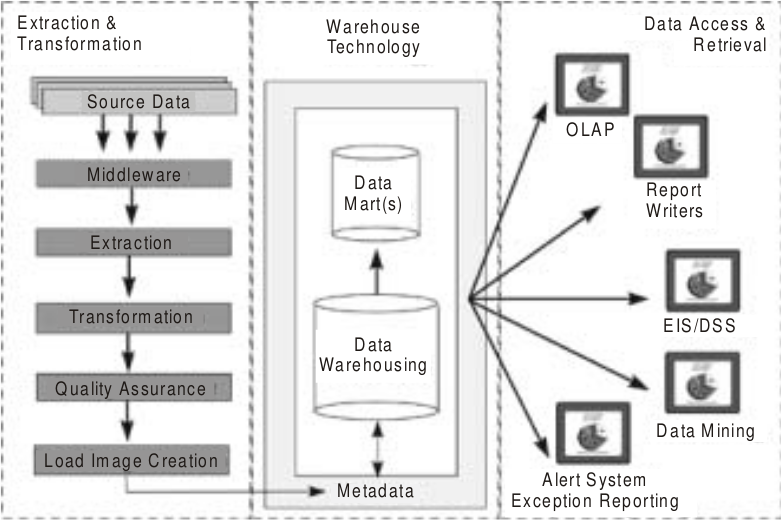
\includegraphics[scale=0.25]{arquitectura}
  
  Arquitectura del Data Warehouse
  \end{center}
}
\end{frame}

\fbckg{white}
\begin{frame}
\pointedsl{¿Qué es OLAP?}
\end{frame}


\fbckg{white}
\begin{frame}
\misc
{
El \textbf{procesamiento analítico en línea} (On-Line Analytical Processing, OLAP) es una solución utilizada en el campo de la inteligencia de negocios, cuyo objetivo es permitir la consulta de grandes cantidades de datos de forma eficiente y sencilla.
}
\end{frame}

\fbckg{white}
\begin{frame}
\misc
{
El concepto OLAP puede definirse mediante 5 palabras: Análisis Rápido de Información Compartida Multidimensional, (Fast Analysis of Shared Multidimensional Information, o FASMI).
}
\end{frame}

\fbckg{white}
\begin{frame}
\misc
{
\begin{itemize}
  \item \textbf{Rápida}: el sistema está dirigido a proporcionar la mayoría de las respuestas a los usuarios en pocos segundos.
  \item \textbf{Análisis}: el sistema puede hacer frente a cualquier lógica de negocio y análisis estadístico que sea relevante para el usuario, en forma relativamente sencilla.
  \item \textbf{Compartida}: significa que el sistema implementa todos los requisitos de seguridad de la confidencialidad.
  \item \textbf{Multidimensionalidad}: el sistema debe proveer una vista conceptual multidimensional de los datos.
  \item \textbf{Información}: se refiere a todos los datos y a la información derivada, que sea relevante para la aplicación.
\end{itemize}
}
\end{frame}


\fbckg{white}
\begin{frame}
\pointedsl{{\LARGE Reglas de Codd}}
\end{frame}

\fbckg{white}
\begin{frame}
\itemized{
\item \textbf{Visión multidimensional}
}
\end{frame}

\fbckg{white}
\begin{frame}
\itemized{
\item \textbf{Visión multidimensional}
\item \textbf{Manipulación intuitiva de los datos}
}
\end{frame}

\fbckg{white}
\begin{frame}
\itemized{
\item \textbf{Visión multidimensional}
\item \textbf{Manipulación intuitiva de los datos}
\item \textbf{Accesibilidad}
}
\end{frame}

\fbckg{white}
\begin{frame}
\itemized{
\item \textbf{Visión multidimensional}
\item \textbf{Manipulación intuitiva de los datos}
\item \textbf{Accesibilidad}
\item \textbf{Soporte multi-usuario}
}
\end{frame}

\fbckg{white}
\begin{frame}
\itemized{
\item \textbf{Visión multidimensional}
\item \textbf{Manipulación intuitiva de los datos}
\item \textbf{Accesibilidad}
\item \textbf{Soporte multi-usuario}
\item \textbf{Información separada del origen de datos}
}
\end{frame}

\fbckg{white}
\begin{frame}
\itemized{
\item \textbf{Visión multidimensional}
\item \textbf{Manipulación intuitiva de los datos}
\item \textbf{Accesibilidad}
\item \textbf{Soporte multi-usuario}
\item \textbf{Información separada del origen de datos}
\item \textbf{Flexibilidad ante valores nulos}
}
\end{frame}

\fbckg{white}
\begin{frame}
\itemized{
\item \textbf{Visión multidimensional}
\item \textbf{Manipulación intuitiva de los datos}
\item \textbf{Accesibilidad}
\item \textbf{Soporte multi-usuario}
\item \textbf{Información separada del origen de datos}
\item \textbf{Flexibilidad ante valores nulos}
\item \textbf{Rendimiento uniforme}
}
\end{frame}

\fbckg{white}
\begin{frame}
\itemized{
\item \textbf{Visión multidimensional}
\item \textbf{Manipulación intuitiva de los datos}
\item \textbf{Accesibilidad}
\item \textbf{Soporte multi-usuario}
\item \textbf{Información separada del origen de datos}
\item \textbf{Flexibilidad ante valores nulos}
\item \textbf{Rendimiento uniforme}
\item \textbf{Dimensiones y niveles de agregación ilimitados}
}
\end{frame}

\fbckg{white}
\begin{frame}
\pointedsl{Jerarquías}
\end{frame}

\fbckg{white}
\begin{frame}
\misc
{
  Las \textbf{jerarquías} se utilizan para especificar en menor o mayor detalle los datos contenidos en la dimensión. Las jerarquías son de mucha utilidad a la hora de calcular valores "agregados"\\ \ \\ \ \\

  \underline{Ejemplos:}
  \begin{center}
  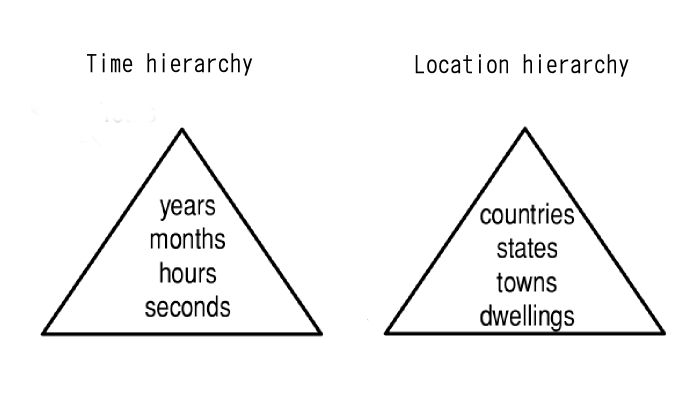
\includegraphics[scale=0.3]{jerarquias}
  \end{center}
}
\end{frame}


\fbckg{white}
\begin{frame}
\pointedsl{\LARGE{Agregaciones}}
\end{frame}

\fbckg{white}
\begin{frame}
\misc
{
Un \textbf{agregado} es un resumen precalculado, almacenado en un DW, por lo general en un esquema separado.
Los agregados típicamente se calculan en base a los registros en el nivel más detallado (o base) de su jerarquía. Se utilizan para mejorar el rendimiento de aquellas consultas que requieren sólo de datos sumarizados, o de alto nivel.
}
\end{frame}

\fbckg{white}
\begin{frame}
\misc
{
\textbf{Ejemplo:}
\begin{figure}
        \centering
        \begin{subfigure}[b]{0.5\textwidth}
                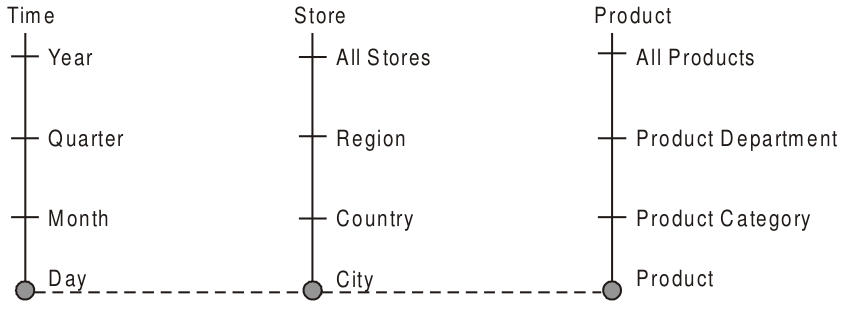
\includegraphics[width=\textwidth]{ej1_agregados}

                \textbf{Esquema de nivel base} que usa la parte inferior del nivel de je-rarquías dimensionales.
        \end{subfigure}%
        ~ \quad
        \begin{subfigure}[b]{0.5\textwidth}
                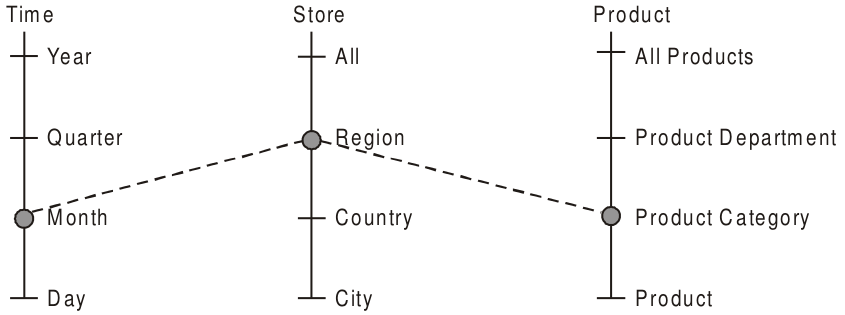
\includegraphics[width=\textwidth]{ej2_agregados}
                
                \textbf{Esquema agregado}, que resulta en datos en un nivel más alto en la jerarquía dimensional.
        \end{subfigure}
\end{figure}

Los \textbf{esquemas agregados} proporcionan mejoras en el rendimiento, ya que tienen un número significativamente menor de registros,
en relación al esquema que se quiere resumir.

}
\end{frame}

\fbckg{white}
\begin{frame}
\misc
{
El uso más común de los agregados es tomar una dimensión y cambiar su granularidad.
Al cambiar la granularidad de la dimensión, la tabla de hechos tiene que ser parcialmente resumida para adaptarse a la nueva dimensión. Se crean así, nuevas tablas de dimensiones y tablas de hechos, que encajan en este nuevo nivel de granularidad.
}
\end{frame}

\fbckg{white}
\begin{frame}
\misc
{
\textbf{Ejemplo:}

Este esquema copo de nieve, tiene una sola tabla de hechos \textit{Sales}, dos métricas (\textit{units and dollars}) y cuatro tablas de dimensiones (\textit{Product, Mfr, Customer, Time, y Customer}).

\begin{center}
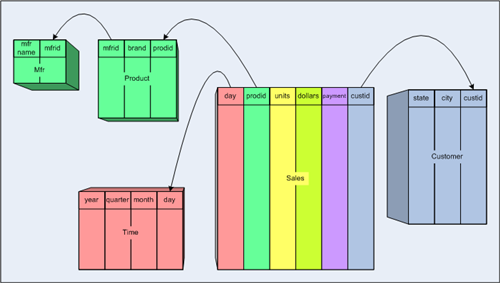
\includegraphics[scale=0.4]{aggregate_tables_1}
\end{center}
}
\end{frame}

\fbckg{white}
\begin{frame}
\misc
{
A partir del esquema anterior, creamos una \textbf{tabla agregada}, que llamamos \textbf{Agg\_1}:
 
\begin{center}
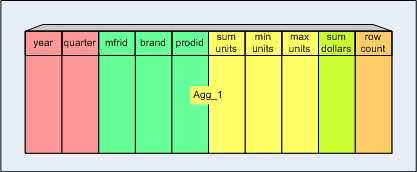
\includegraphics[scale=0.5]{aggregate_tables_2}
\end{center}
}
\end{frame}

\fbckg{white}
\begin{frame}
\misc
{Veamos como se combinaron las columnas del esquema original, en la tabla agregada \textbf{Agg\_1}:

\begin{itemize}
  \item La dimensión \textit{Time} "colapsó" en la tabla de agregación, omitiendo las columnas \textit{month} y \textit{day}.
  \item Las dos tablas de la dimensión \textit{Product} "colapsaron" en la tabla de agregación.
  \item La dimensión \textit{Customer} se "perdió".
  \item Para cada métrica en la tabla de hechos (\textit{units, dollars}), hay uno o más métricas en la tabla de agregación (\textit{sum units, min units, max units, sum dollars}).
  \item También hay una nueva métrica, \textit{row count}, que representa la métrica "conteo".
\end{itemize}
}
\end{frame}


\fbckg{white}
\begin{frame}
\misc
{

Veamos otra prosible tabla agregada, \textbf{Agg\_2}:

\begin{center}
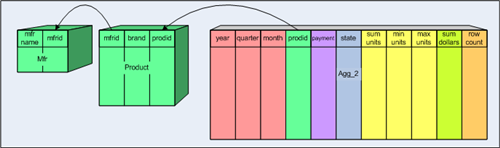
\includegraphics[scale=0.5]{aggregate_tables_3}
\end{center}

Varias dimensiones colapsaron: \textit{Time} en el nivel \textit{month}; \textit{Customer} en el nivel \textit{state};
y \textit{Payment Method} a nivel \textit{payment method}. Mientras que la dimensión \textit{Product} se mantuvo tal como estaba en el esquema original.}
\end{frame}


\fbckg{white}
\begin{frame}
\misc
{
Tener datos agregados en el modelo dimensional hace que el entorno sea más complejo.
Para que esta complejidad adicional sea transparente al usuario, se utiliza una funcionalidad conocida como \textit{navegación de agregados},
la cual es implementada por el motor OLAP, para consultar las tablas dimensionales y de hecho, con el nivel de granularidad correcto.
}
\end{frame}

\fbckg{white}
\begin{frame}
\pointedsl{\LARGE{Hipercubo de datos}}
\end{frame}

\fbckg{white}
\begin{frame}
\misc
{
OLAP utiliza \textbf{hipercubos} o \textbf{cubos}, de la misma manera que las bases de datos utilizan tablas. Toda la navegación, informes y análisis se hacen en términos de hipercubos.

Por lo tanto, un "cubo" de datos se refiere a una representación multidimensional de los datos en dicha forma (obviamente, sólo en el espacio tridimensional).
}
\end{frame}


\fbckg{white}
\begin{frame}
\misc
{
Construiremos un cubo, tomando como ejemplo el siguiente conjunto de datos:
\begin{center}
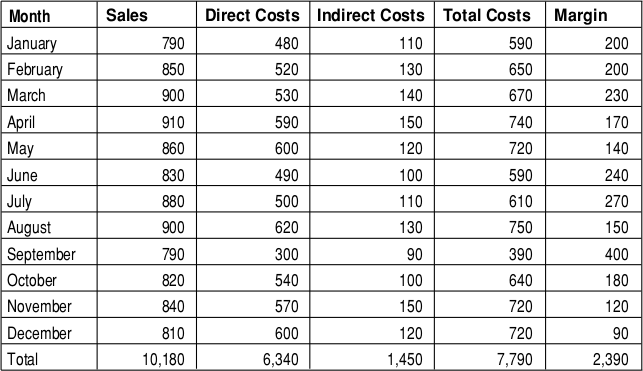
\includegraphics[scale=0.4]{cube_1}
\end{center}
}
\end{frame}


\fbckg{white}
\begin{frame}
\misc
{
Decimos que \textit{sales}, \textit{costs}, y \textit{margin} representan \textbf{variables}.

Si alguien pregunta, "¿Qué estás midiendo?".

Le respondemos, "ventas, costos y márgenes".

Ante la pregunta, "¿De dónde consigue sus datos?", o "¿con qué frecuencia está haciendo mediciones?".

Responderíamos, "Estamos siguiendo las ventas mensuales." Los meses representan la organización de los datos.

Entonces, hay dos dimensiones, el \textit{tiempo} y las \textit{variables}.
\newline

Este enfoque de \textbf{dimensiones genéricas}, utiliza invariable- mente una \textbf{dimensión de hechos}, o \textbf{variables}.
Tratar a los \textbf{hechos} como miembros de una dimensión, implica la creación de una \textbf{dimensión de datos}. 
}
\end{frame}

\fbckg{white}
\begin{frame}
\misc
{
¿Qué sucede cuando añadimos una tercera dimensión llamada \textit{products} (productos)?.
Tenemos un cubo.

\begin{center}
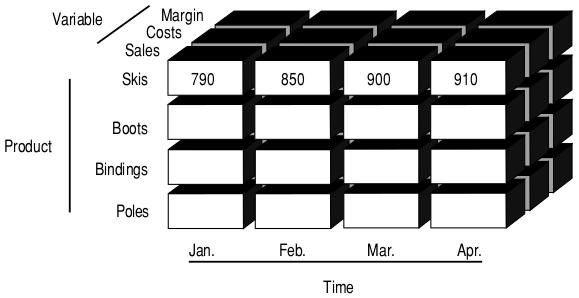
\includegraphics[scale=0.4]{cube_2}
\end{center}
}
\end{frame}

\fbckg{white}
\begin{frame}
\misc
{
El conjunto de datos tridimensionales, que consiste de \textit{variables}, \textit{time}, y \textit{products}, se puede mostrar en una pantalla en términos de: \textbf{fila}, \textbf{columna} y \textbf{página}.

\begin{center}
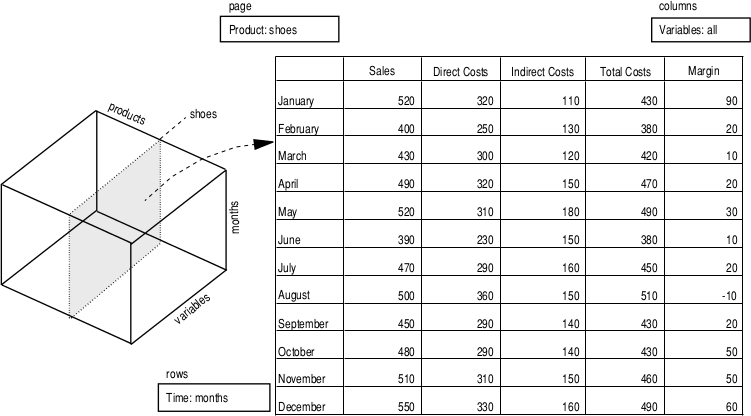
\includegraphics[scale=0.32]{cube_3}
\end{center}
}
\end{frame}


\fbckg{white}
\begin{frame}
\misc
{
¿Qué pasa si intentamos añadir una cuarta dimensión \textit{tienda}, al cubo?. El cubo como metáfora visual se rompe.
\newline

Presentamos una nueva estructura para representar datos, o eventos generadores de datos, que es capaz de reproducir cualquier número de dimensiones.

La llamamos, \textbf{estructura de tipo multidimensional} (\textit{Multidi- mensional Type Structures}, o MTS).

Cada dimensión está representada por una línea. Cada miembro dentro de una dimensión está representado por un intervalo, dentro del segmento correspondiente.
}
\end{frame}

\fbckg{white}
\begin{frame}
\misc
{
Siguiendo el ejemplo, tenemos tres líneas:

Una para el \textit{tiempo}, una de los \textit{productos}, y por último, una para las \textit{variables}.

Cualquier unión de los intervalos de cada una de los tres líneas, está conectada a un evento y a un elemento del cubo.

\begin{center}
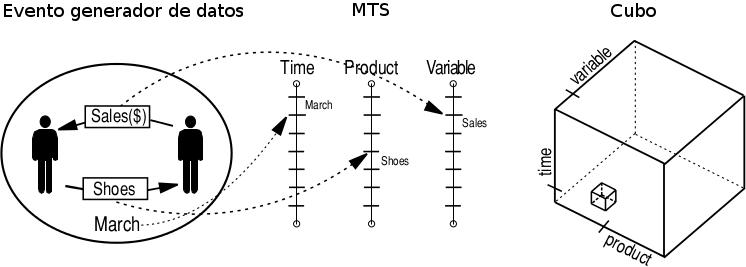
\includegraphics[scale=0.3]{cube_4}
\end{center}
}
\end{frame}

\fbckg{white}
\begin{frame}
\pointedsl{\large{Hipercubos en una pantalla}}
\end{frame}

\fbckg{white}
\begin{frame}
\misc
{
Para ver los datos en la pantalla, tenemos que mapear múltiples dimensiones lógicas en dos dimensiones físicas

(la pantalla).
}
\end{frame}


\fbckg{white}
\begin{frame}
\misc
{
Mapear dos dimensiones en una dimensión, implica crear una versión unidimensional de las dos dimensiones.
El método típico consiste en anidar una dimensión dentro de la otra.

\begin{figure}
        \centering
        \begin{subfigure}[b]{0.55\textwidth}
                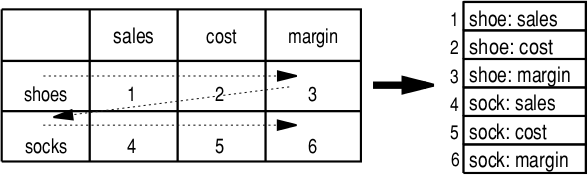
\includegraphics[width=\textwidth]{cube_5}

                Variables anidadas en productos.
        \end{subfigure}
        
        
        \ \hfil
        
        
        \begin{subfigure}[b]{0.55\textwidth}
                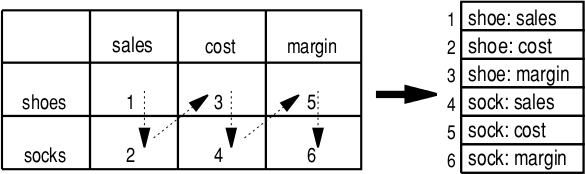
\includegraphics[width=\textwidth]{cube_6}
                
                Productos anidados en variables
        \end{subfigure}
\end{figure}
}
\end{frame}

\fbckg{white}
\begin{frame}
\misc
{
Efectos de combinar dimensiones:

{
\begin{figure}
        \centering
        \begin{subfigure}[b]{0.4\textwidth}
          $\textendash$ Cambia la forma de los datos visibles. La longi-tud de una lista unidimensional es igual al producto de las longitudes de cada una de las dos dimensiones.
          
          $\textendash$ Cambia el conjunto de vecinos que rodean cualquier punto.
        \end{subfigure}
        ~
        \begin{subfigure}[b]{0.4\textwidth}
          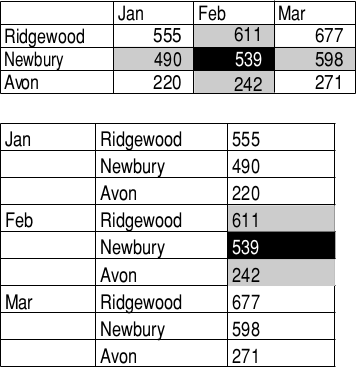
\includegraphics[width=\textwidth]{cube_7}
        \end{subfigure}
\end{figure}
}
}
\end{frame}

\fbckg{white}
\begin{frame}
\misc
{
Siguiendo el ejemplo, que ahora consiste de: \textit{products}, \textit{times}, \textit{stores}, \textit{customers}, \textit{variables}, y \textit{scenarios};
vemos una posible representación, en base a filas, columnas y páginas:
\begin{figure}
        \centering
        \begin{subfigure}[b]{0.5\textwidth}
                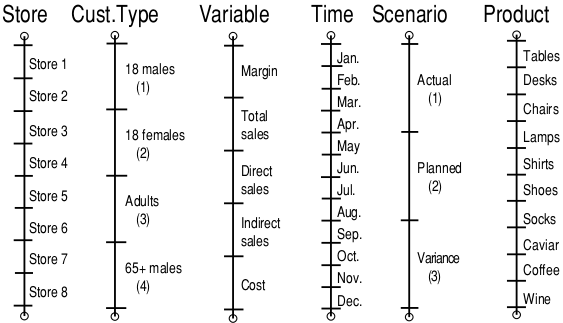
\includegraphics[width=\textwidth]{cube_8}
        \end{subfigure}%
        ~
        \begin{subfigure}[b]{0.55\textwidth}
                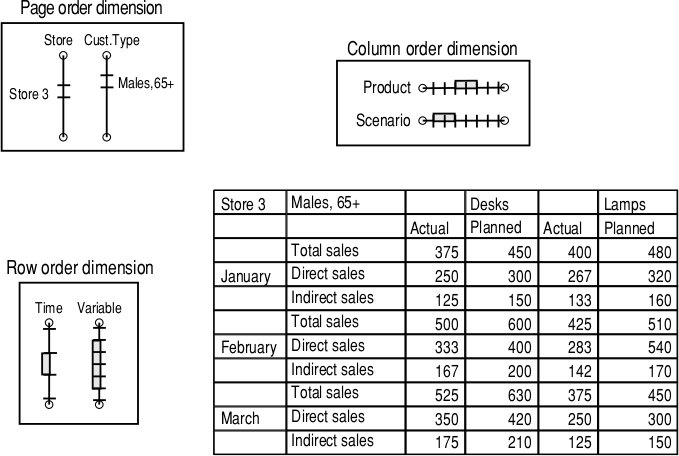
\includegraphics[width=\textwidth]{cube_9}
        \end{subfigure}
\end{figure}
}
\end{frame}

\fbckg{white}
\begin{frame}
\misc
{
La capacidad de cambiar fácilmente las vistas de los mismos datos, mediante la reconfiguración de cómo se muestran las dimensiones, es uno de los grandes beneficios
que proveen los sistemas multidimensionales, a la navegación de los usuarios finales.
Esto se debe a la separación de la estructura de datos (MTS), de su visualización (grilla multidimensional).
}
\end{frame}


\fbckg{white}
\begin{frame}
\misc
{
Hay algunas reglas básicas que hay que tener en cuenta en el análisis de datos multidimensionales:
\begin{itemize}
  \item Debe tratar de utilizar páginas. Esto ayuda a maximizar el grado en que todo en la pantalla es relevante.
  \item Cuando necesita anidar múltiples dimensiones a través de las filas y columnas, generalmente es mejor anidar más dimensiones a través de las columnas que a través de las filas, ya que suele haber mas espacio vertical en la pantalla, que horizontal.
  \item Antes de decidir cómo mostrar la información en la pantalla, pregúntese "¿Qué quiero mirar?", o "¿Qué estoy tratando de comparar?".
\end{itemize}
}
\end{frame}

\fbckg{white}
\begin{frame}
\misc
{ Vista clásica OLAP:
\begin{center}
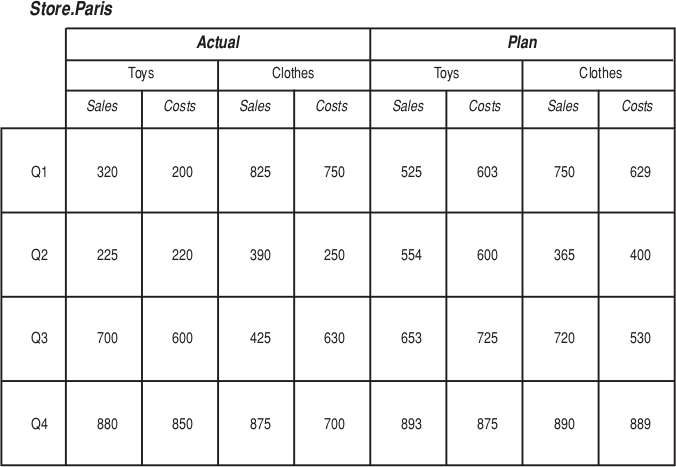
\includegraphics[scale=0.4]{cube_10}
\end{center}
}
\end{frame}


\fbckg{white}
\begin{frame}
\pointedsl{Operaciones}
\end{frame}


\fbckg{white}
\begin{frame}
\misc
{
  \underline{Slice:}\\
En esta operación seleccionamos un valor particular de una de las dimensiones del cubo, buscando así quedarnos con una “rebanada” del cubo.
}
\end{frame}

\fbckg{white}
\begin{frame}
\misc
{
  \underline{Slice:}
  \begin{center}
  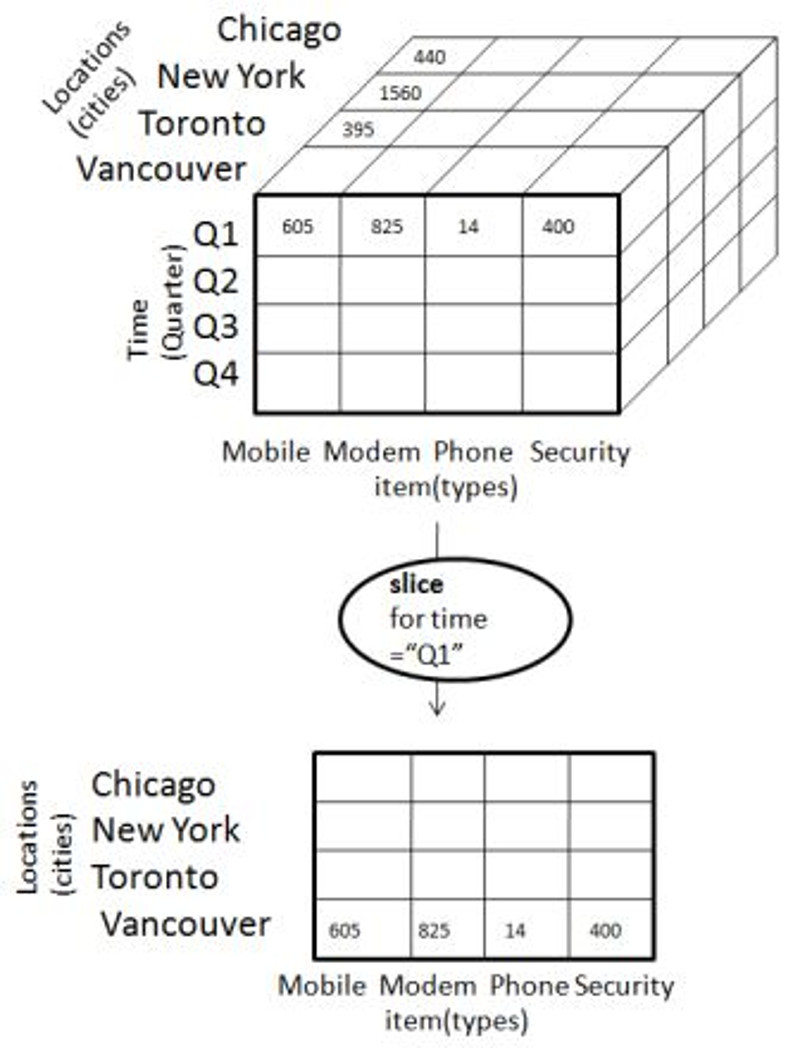
\includegraphics[scale=0.15]{slice}
  \end{center}
}
\end{frame}


\fbckg{white}
\begin{frame}
\misc
{
  \underline{Dice:}\\
  Seleccionar valores específicos para 2 o más dimensiones de las que se visualizan
  y con esto obtener un subcubo del cubo original.
}
\end{frame}

\fbckg{white}
\begin{frame}
\misc
{
  \underline{Dice:}
  \begin{center}
  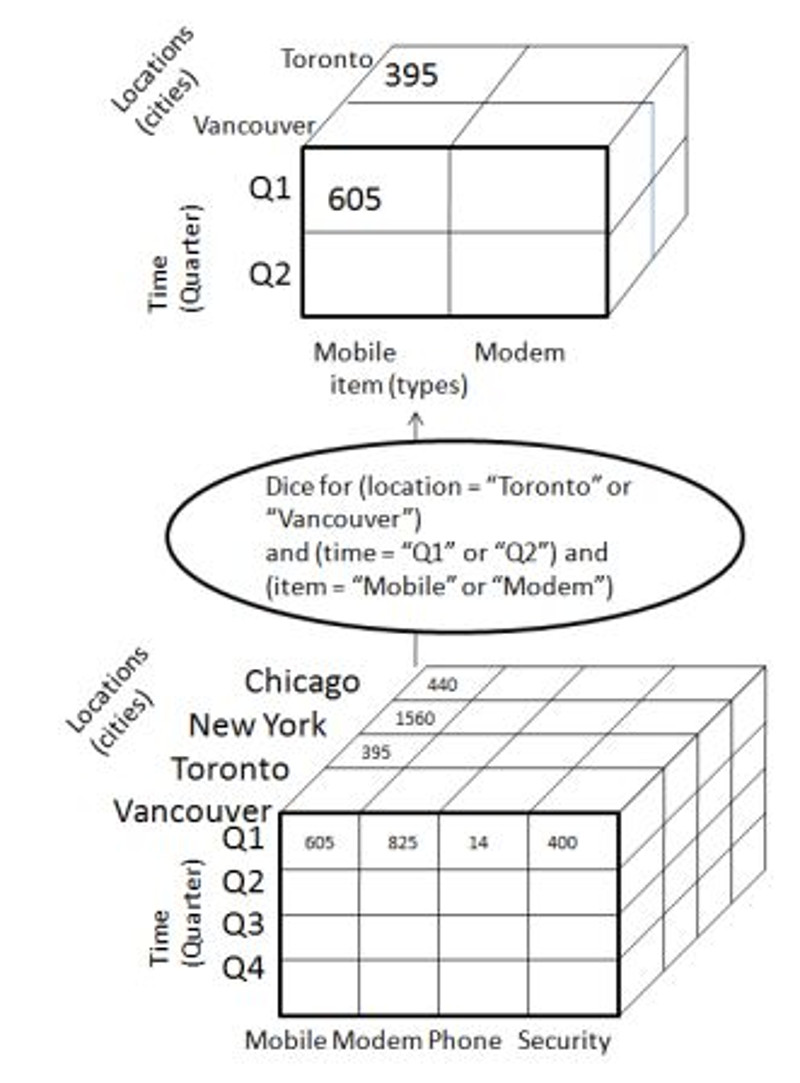
\includegraphics[scale=0.15]{dice}
  \end{center}
}
\end{frame}


\fbckg{white}
\begin{frame}
\misc
{
  \underline{Drill Down:}\\
Esta operación lo que busca es ofrecer más detalle respecto de la información que actualmente se puede visualizar. Esto se puede lograr de dos formas, bajando un nivel en la jerarquía de una dimensión particular o agregando una dimensión para dar aún mas información sobre el contexto.
}
\end{frame}

\fbckg{white}
\begin{frame}
\misc
{
  \underline{Drill Down:}
  \begin{center}
  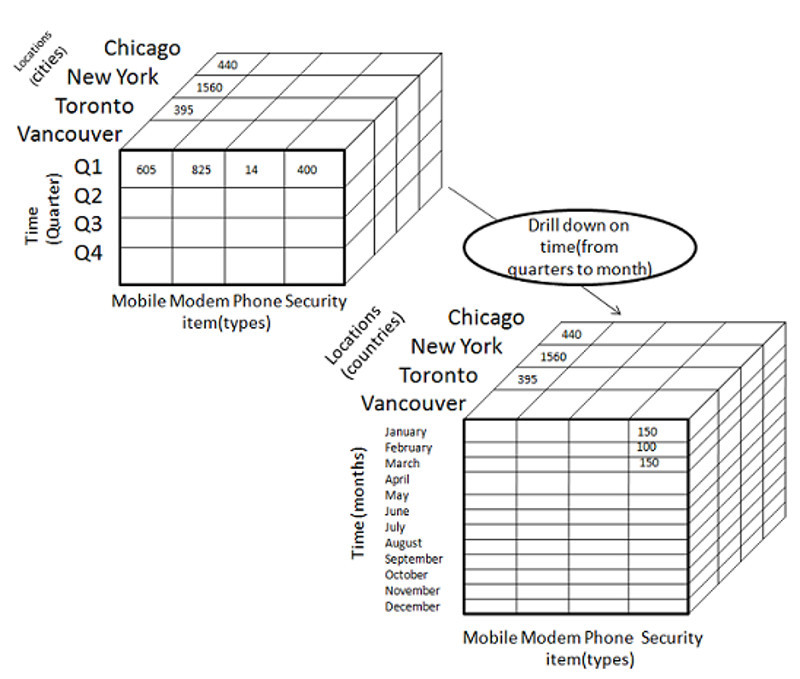
\includegraphics[scale=0.5]{drill_down}
  \end{center}
}
\end{frame}


\fbckg{white}
\begin{frame}
\misc
{
  \underline{Drill Up:}\\
A diferencia de la anterior operación lo que queremos lograr es visualizar menos información, abstraernos un poco más, lo cual puede realizarse subiendo un nivel en la jerarquía de una dimensión o eliminando alguna de las dimensiones.

}
\end{frame}

\fbckg{white}
\begin{frame}
\misc
{
  \underline{Drill Up:}
  \begin{center}
  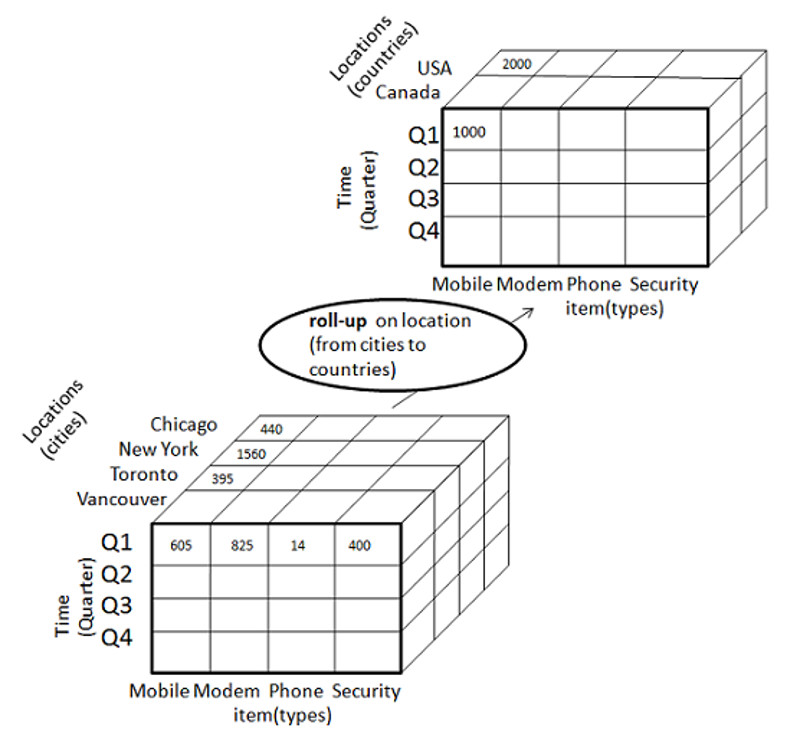
\includegraphics[scale=0.2]{drill_up}
  \end{center}
}
\end{frame}


\fbckg{white}
\begin{frame}
\misc
{
  \underline{Pivot:}\\
Aplicando esta operación ofrecemos al usuario una presentación alternativa de la información rotando los ejes de datos.
}
\end{frame}

\fbckg{white}
\begin{frame}
\misc
{
  \underline{Pivot:}
  \begin{center}
  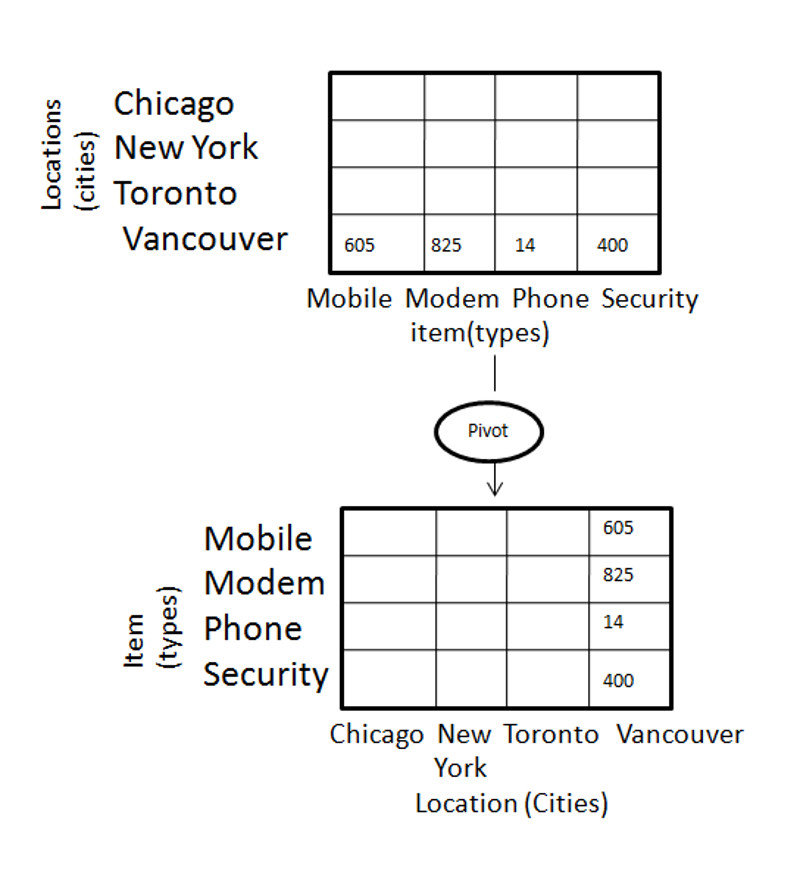
\includegraphics[scale=0.3]{pivot}
  \end{center}
}
\end{frame}

\fbckg{white}
\begin{frame}
\pointedsl{ROLAP}
\end{frame}

\fbckg{white}
\begin{frame}
\misc
{
 El \textbf{procesamiento analítico relacional en línea}, (relational online analytical processing, ROLAP) se trata de sistemas y herramientas OLAP construidos sobre una base de datos relacional (RDB). Las ventajas de este modelo es que puede manejar una gran cantidad de datos y puede aprovechar todas las funcionalidades de la base de datos relacionales. Las desventajas son que el rendimiento es lento, y cada informe ROLAP es una consulta SQL, con lo cual está limitado por las funcionalidades de SQL.
}
\end{frame}

\fbckg{white}
\begin{frame}
\misc
{
  \begin{center}
  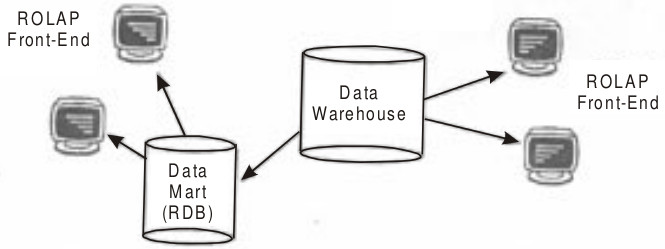
\includegraphics[scale=0.4]{RDB&MDDB}
  
  Bases de datos relacionales
  \end{center}
}
\end{frame}


\fbckg{white}
\begin{frame}
\pointedsl{MOLAP}
\end{frame}

\fbckg{white}
\begin{frame}
\misc
{
El \textbf{procesamiento analítico multidimensional en línea}, (multidimensional online analytical processing, MOLAP) consiste en herramientas que se ejecutan sobre una base de datos multidimensional (MDDB). La ventaja principal de este modelo es que proporciona un
gran rendimiento de consultas, dado que se pre-computan los datos en el cubo, cuando éste es creado. Sin embargo este modelo solo puede manejar una cantidad limitada de datos, ya que el cubo no se puede derivar de un gran volumen de datos.
}
\end{frame}

\fbckg{white}
\begin{frame}
\misc
{
  \begin{center}
  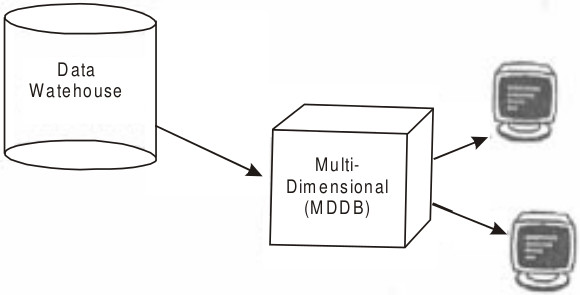
\includegraphics[scale=0.4]{RDB&MDDB2}
  
  Bases de datos multidimensionales
  \end{center}
}
\end{frame}


\fbckg{white}
\begin{frame}
\pointedsl{MDDB vs. RDB}
\end{frame}

\fbckg{white}
\begin{frame}
\misc
{
\begin{itemize}
  \item \textbf{Bases de datos multidimensionales}: las MDDBs alma- cenan los datos en un "hipercubo", es decir, una matriz de almacenamiento multidimensional optimizada.

\item \textbf{Bases de datos relacionales}: las RDBs guardan los datos como tablas, con filas y columnas que no mapean directamente con la vista multidimensional que tienen los usuarios de los datos.
\end{itemize}
}
\end{frame}

\fbckg{white}
\begin{frame}
\misc
{
\begin{itemize}
  \item \textbf{Tamaño}: las MDDBs están, generalmente limitados por el tamaño de los datos, aunque el límite en el tamaño ha ido aumentando gradualmente a lo largo de los años.
  \item \textbf{Volatilidad de los datos de origen}: las RDBs tratan mejor la alta volatilidad de los datos. Los datos multidi- mensionales en hipercubos generalmente tardan mucho en cargarse y actualizarse.
  \item \textbf{Protección de la inversión}: La mayoría de las empresas ya han realizado importantes inversiones en tecnología relaciona.
  El uso continuado de estas herramientas y habilidades para otro propósito proporciona un rendimiento adicional de la inversión.
\end{itemize}
}
\end{frame}

\fbckg{white}
\begin{frame}
\pointedsl{HOLAP}
\end{frame}

\fbckg{white}
\begin{frame}
\misc
{
El \textbf{procesamiento analítico en línea híbrido} (Hybrid Online Analytical Process, HOLAP) es una combinación de ROLAP y MOLAP. HOLAP permite almacenar una parte de los datos como en un sistema MOLAP y el resto como en uno ROLAP.
}
\end{frame}

\fbckg{white}
\begin{frame}
\misc
{
  \begin{center}
  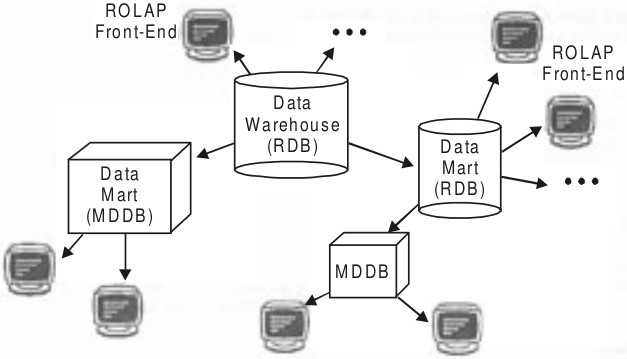
\includegraphics[scale=0.4]{RDB&MDDB3}
  
  Bases de datos de relaciones, y multidimensionales.
  \end{center}
}
\end{frame}

\fbckg{white}
\begin{frame}
\pointedsl{{\LARGE Charla concluida}}
\end{frame}
\end{document}
